\scanpage{76}
qui \uline{généralise le th. de pureté relatif}
[et se déduit d'ailleurs du th de dualité globale --- cela devrait être explicité dans SGA \deleted{\unsure{4|5}}].
\margin{\figure{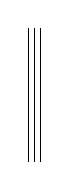
\begin{tikzpicture}\draw (0,0)--(0,1.7);\draw (.08,0)--(.08,1.7);\draw (.16,0)--(.16,1.7);\end{tikzpicture}}}
Se réduit aux formules
\[
\underline H^i_Y(f^*(G))=
\begin{cases}
0 & i\ne2d\\
g^*(G)\otimes T_{Y/X}^{-1} & \text{si }i=2d
\end{cases}
\]

Cet isomorphisme se généralise donc au cas d'un $G^\bullet$ :
\[
\mathbb{R}g^!(G^\bullet)\simeq \mathbb{R}i^!(\mathbb{R}f^!(G^\bullet))
\]
On en déduit un hom canonique
\[
\deleted{\unsure{\mathbb{R}_!f}(\mathbb{R}g^!(G^\bullet))\longrightarrow \mathbb{R}^!f}
\]
\[
\mathbb{R}_!i_*(\mathbb{R}g^!(G^\bullet))\mathbin{\unsure{-|\longrightarrow}}\mathbb{R}f^!(G^\bullet)
\]
d'où en appliquant $\mathbb{R}_!f_*$, et utilisant la transitivité
\diagram{\begin{tikzcd}[ampersand replacement=\&,column sep=large]
\mathbb{R}_!g_*(\mathbb{R}g^!(G^\bullet)) \arrow[rr] \arrow[dr,no head,"\operatorname{Tr}_g(G^\bullet)"'] \&\&
\mathbb{R}_!f_*\mathbb{R}f^!(G^\bullet) \arrow[dl,"\operatorname{Tr}_f(G^\bullet)"]\\
\& G^\bullet \&
\end{tikzcd}}
\margin{\unsure{rend} commutatif}
\mspage{75}
